\documentclass[10pt]{beamer}

%Package
\usepackage[utf8]{inputenc}
\usepackage[absolute,overlay]{textpos}
% \usepackage[margin=1in]{geometry}
% \usepackage{amsmath}
% \usepackage{fancyhdr}
% \usepackage{graphicx}
% \usepackage{placeins}
% \usepackage{listings}
% \usepackage{color}
% \usepackage[table,xcdraw]{xcolor}
% \usepackage{ulem} %barrer du texte
% \usepackage{cancel}% barrer dans une expression math (\cancel{})
% \usepackage{pgf,tikz}
% \usepackage{mathrsfs}
% \usepackage{multirow}
%\usepackage{gensymb}
% \usepackage{caption}
% \usepackage{eurosym}% pour le symbole €


\usetheme{metropolis}           % Use metropolis theme
\title{TX - Banc brushless \& Asynchrone}

\date{30 Juin 2016}
\author{Geoffrey Gaillard}
\institute{Université de Technologie de Troyes}

\begin{document}

	\maketitle

	\begin{frame}{Etat de départ du projet}

		\begin{textblock*}{80mm}(10mm,15mm)
			\begin{block}{Banc d'essai} 
				\begin{itemize}
					\item Montage pas fini
					\item Manque des pièces
					\item Pas de câblage
				\end{itemize}
			\end{block}
		\end{textblock*}
		
		\begin{textblock*}{60mm}(67.5mm,15mm)
			\begin{block}{Armoire électrique}
				\begin{itemize}
					\item Aucune armoire réalisée
				\end{itemize}
			\end{block}
		\end{textblock*}

		\begin{textblock*}{90mm}(10mm,55mm)
			\begin{block}{Electronique}
				\begin{itemize}
					\item Montage réalisé pour la lecture du capteur de force
					\item Aucun montage pour le contrôle par arduino
				\end{itemize}
			\end{block}
		\end{textblock*}

	\end{frame}
	
	\section{Electronique}

	\begin{frame}{Commande asynchrone}
		
		\begin{textblock*}{80mm}(25mm,10mm)
			\begin{itemize}
				\item Commande en vitesse du variateur en $0-10VDC$
				\item Création d'un convertisseur PWM $\Rightarrow$ $0-10VDC$
 			\end{itemize}
		\end{textblock*}

		\begin{textblock*}{80mm}(20mm,27mm)
				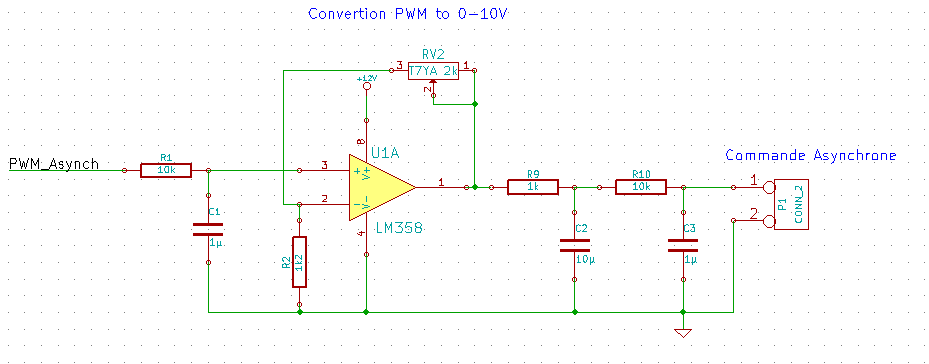
\includegraphics[width=250px]{schema_digt_anolog.png}
		\end{textblock*}

		\begin{textblock*}{80mm}(35mm,60mm)
				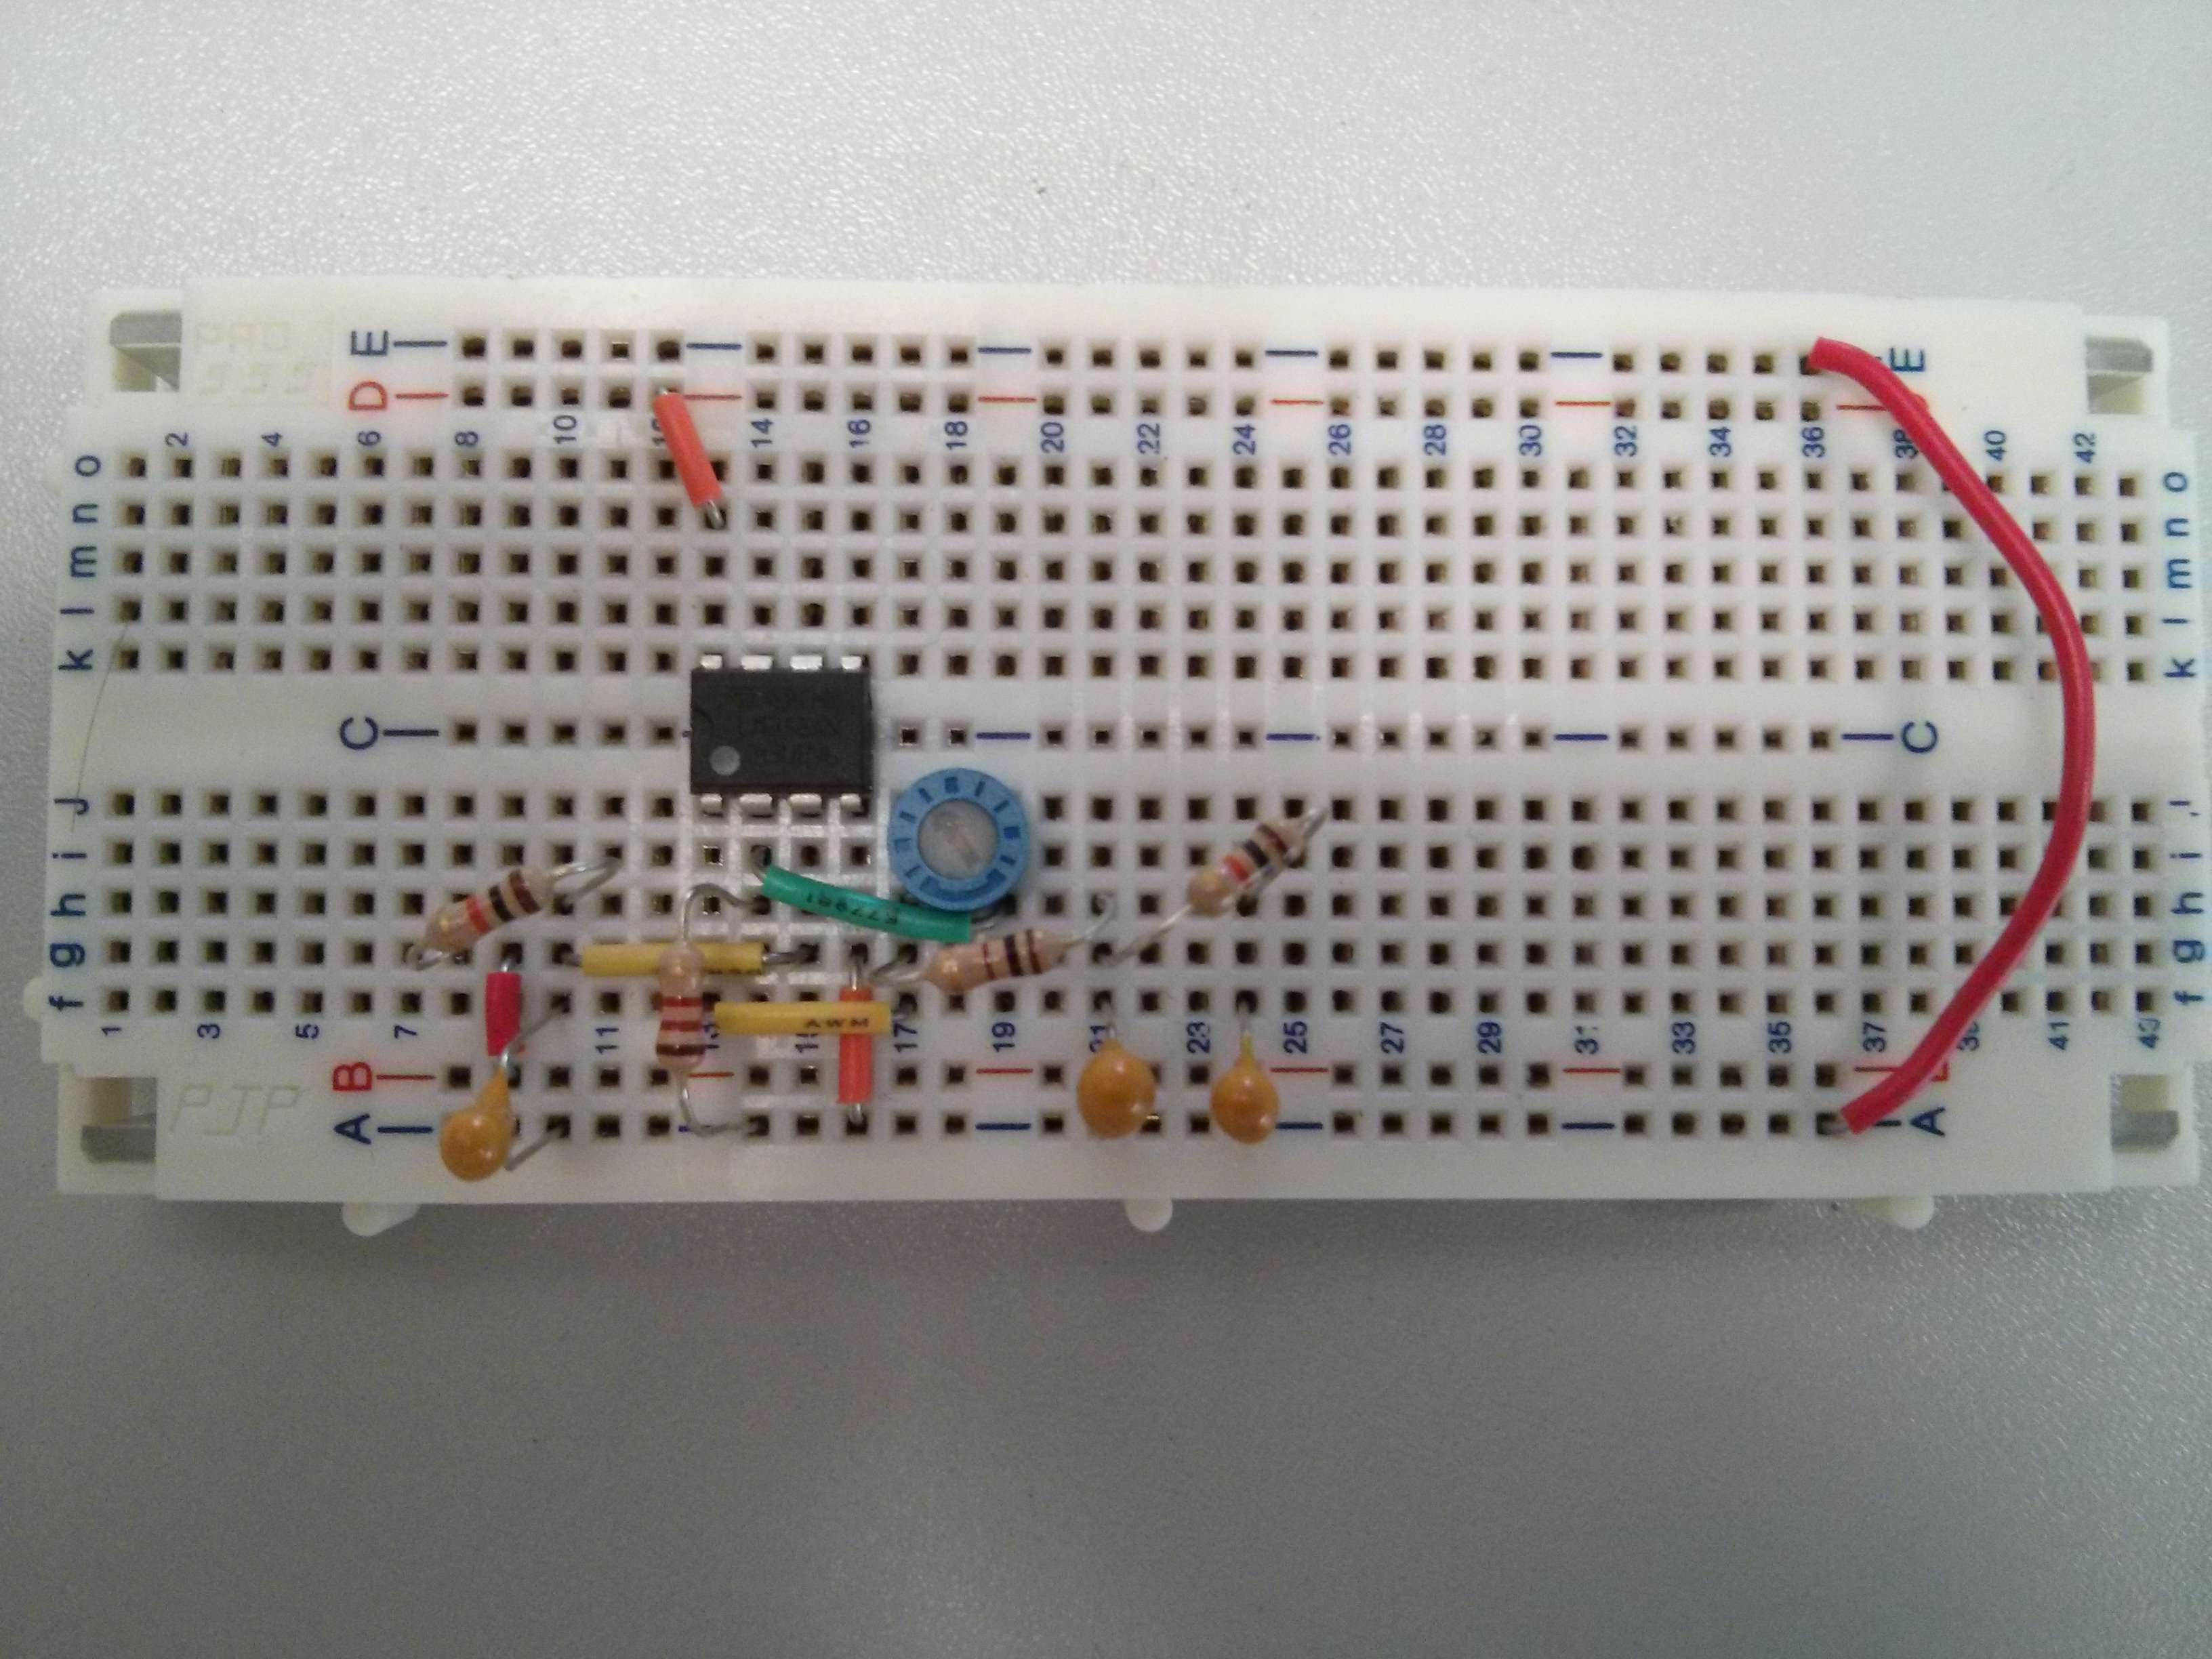
\includegraphics[width=150px]{IMG_20160629_203955.jpg}
		\end{textblock*}
		
	\end{frame}

	\begin{frame}{Asynchrone}
		
		\begin{textblock*}{80mm}(20mm,10mm)
			\begin{itemize}
				\item Commande du sens et du reset
				\item Création d'un circuit de pilotage par transistor
 			\end{itemize}
		\end{textblock*}

		\begin{textblock*}{80mm}(30mm,30mm)
				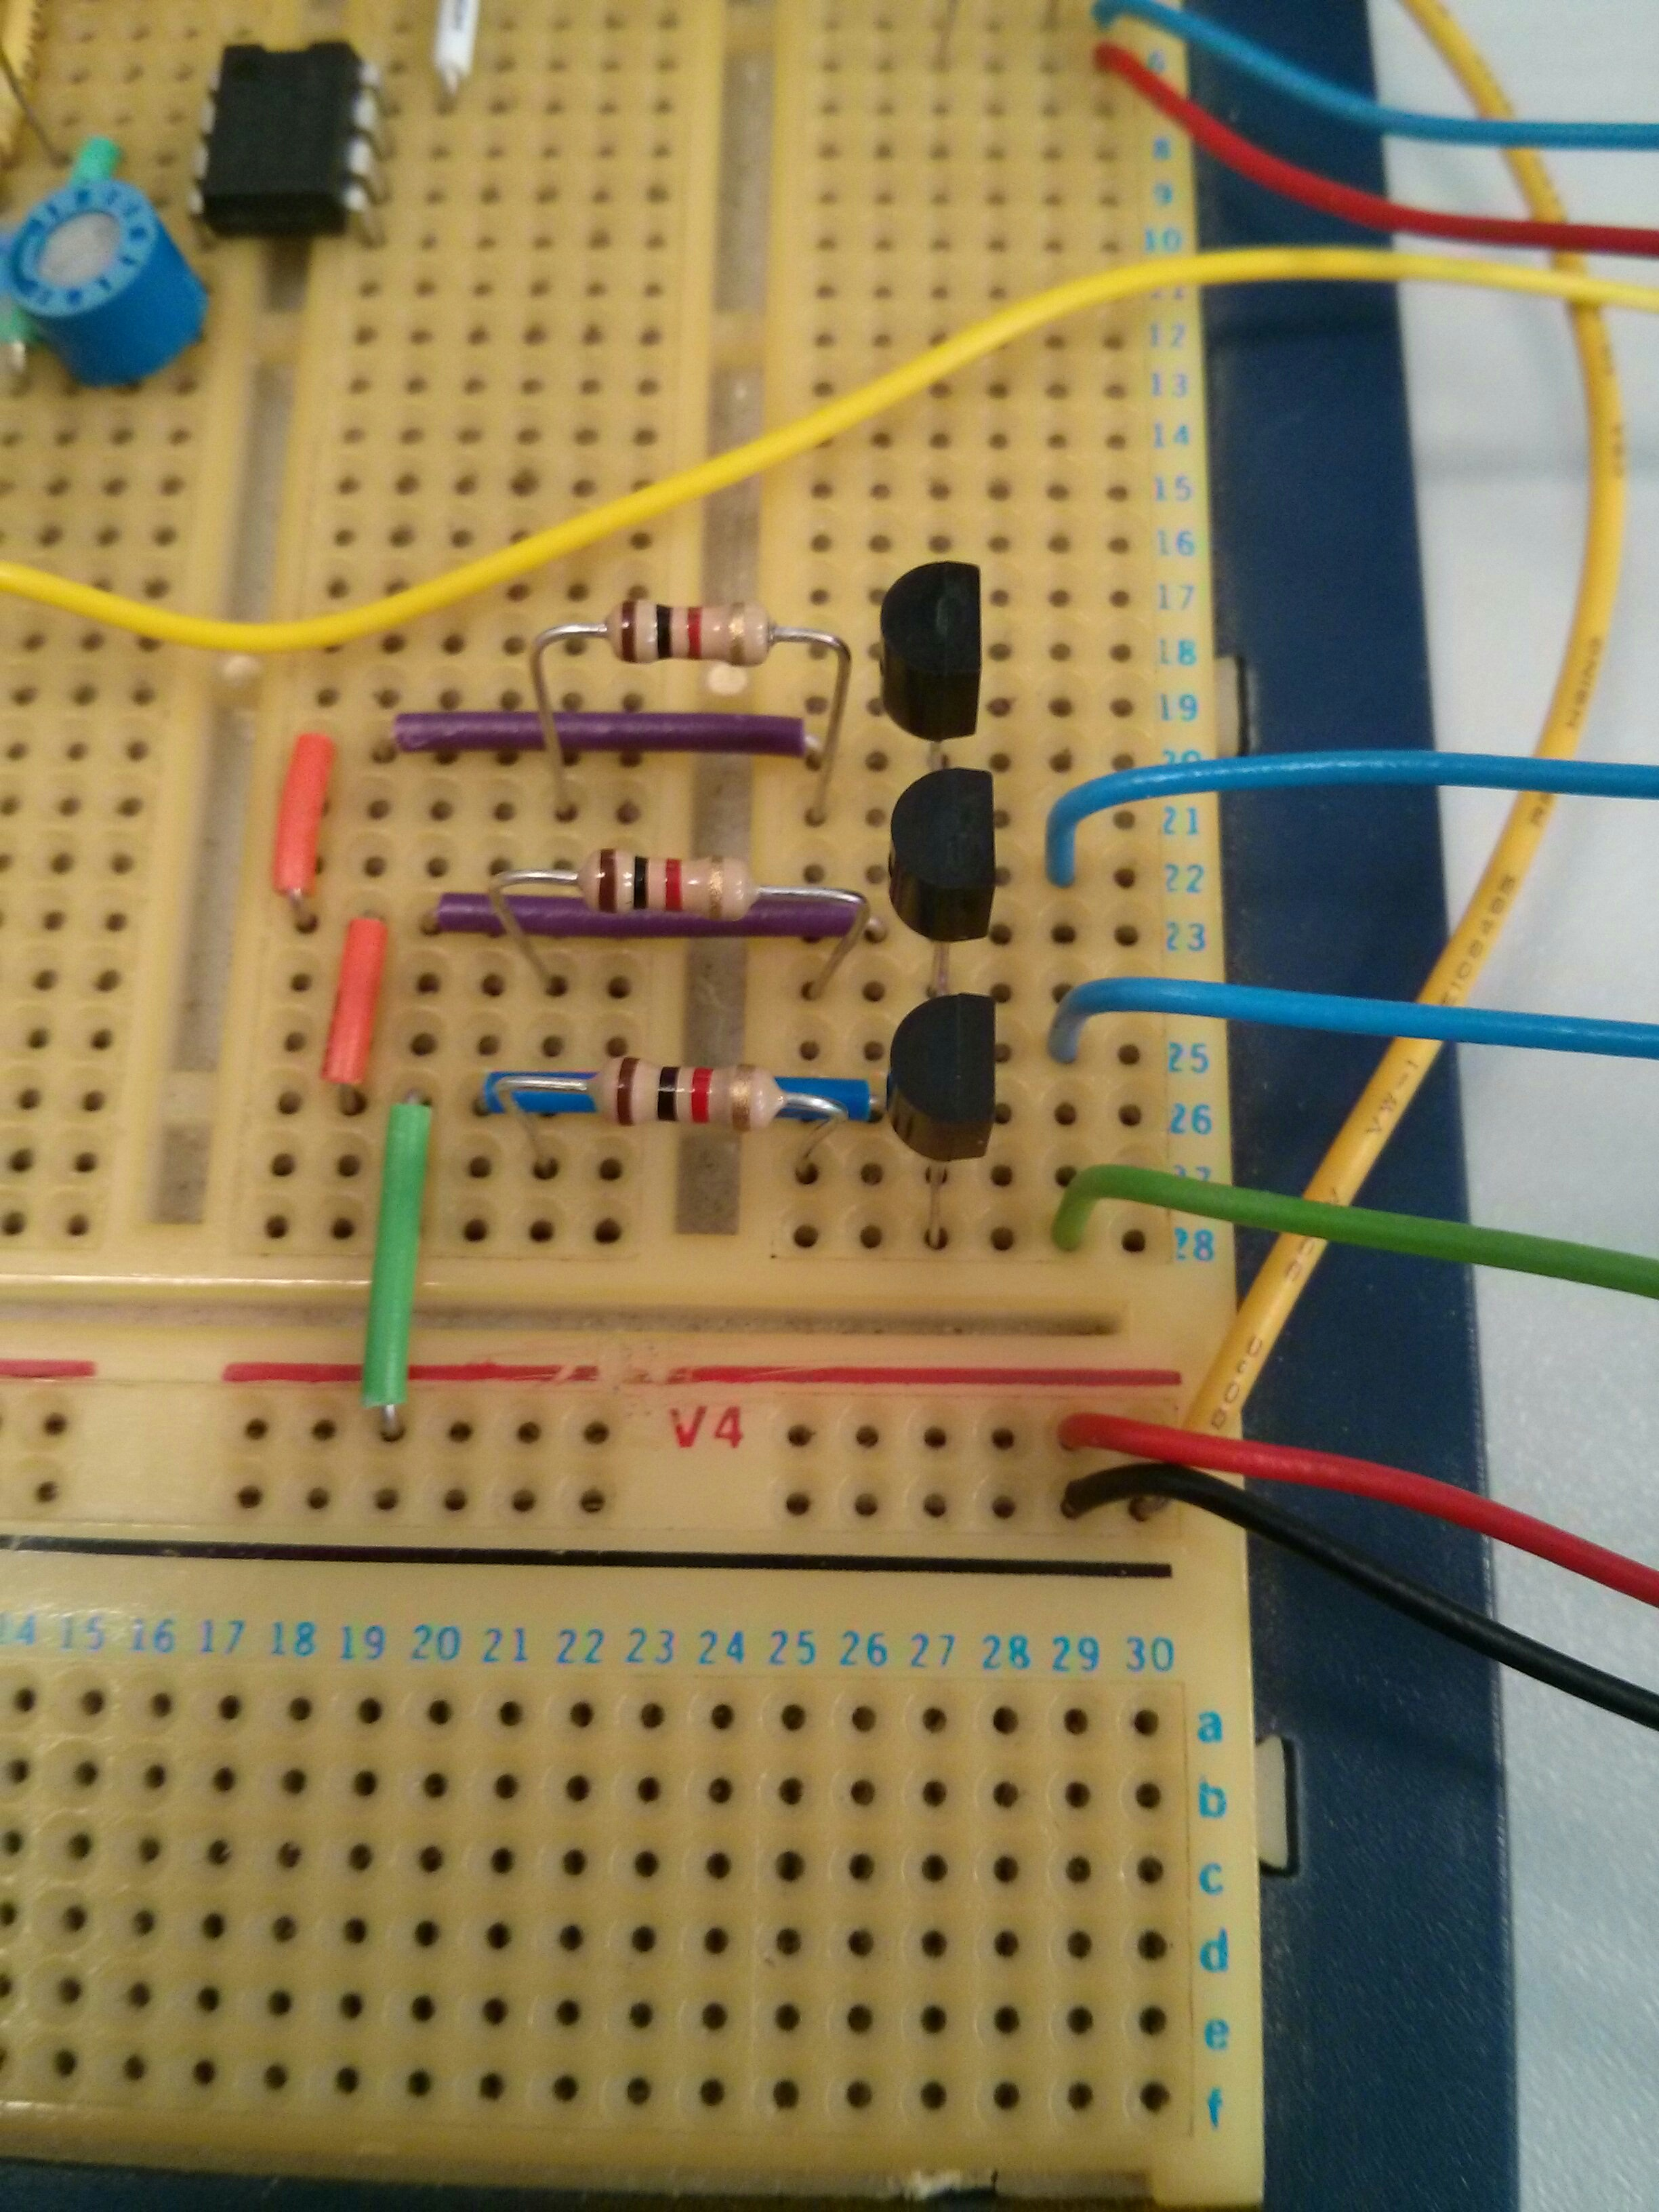
\includegraphics[width=150px]{IMG_20160630_163442.jpg}
		\end{textblock*}
		
	\end{frame}

	\begin{frame}{Brushless}
		
		\begin{textblock*}{100mm}(20mm,30mm)
			\begin{itemize}
				\item Commande de vitesse et de limitation d'intensité en PWM
				\item Commande sens, ON/OFF par digital
				\item Réception encodée et sens réel
 			\end{itemize}
		\end{textblock*}
		
	\end{frame}

	\begin{frame}{Capteur de force}
		
		\begin{textblock*}{80mm}(20mm,10mm)
			\begin{itemize}
				\item Montage réalisé dans une précédente TX
				\item Montage refait pour corriger les erreurs du précédent montage
 			\end{itemize}
		\end{textblock*}

		\begin{textblock*}{80mm}(40mm,30mm)
				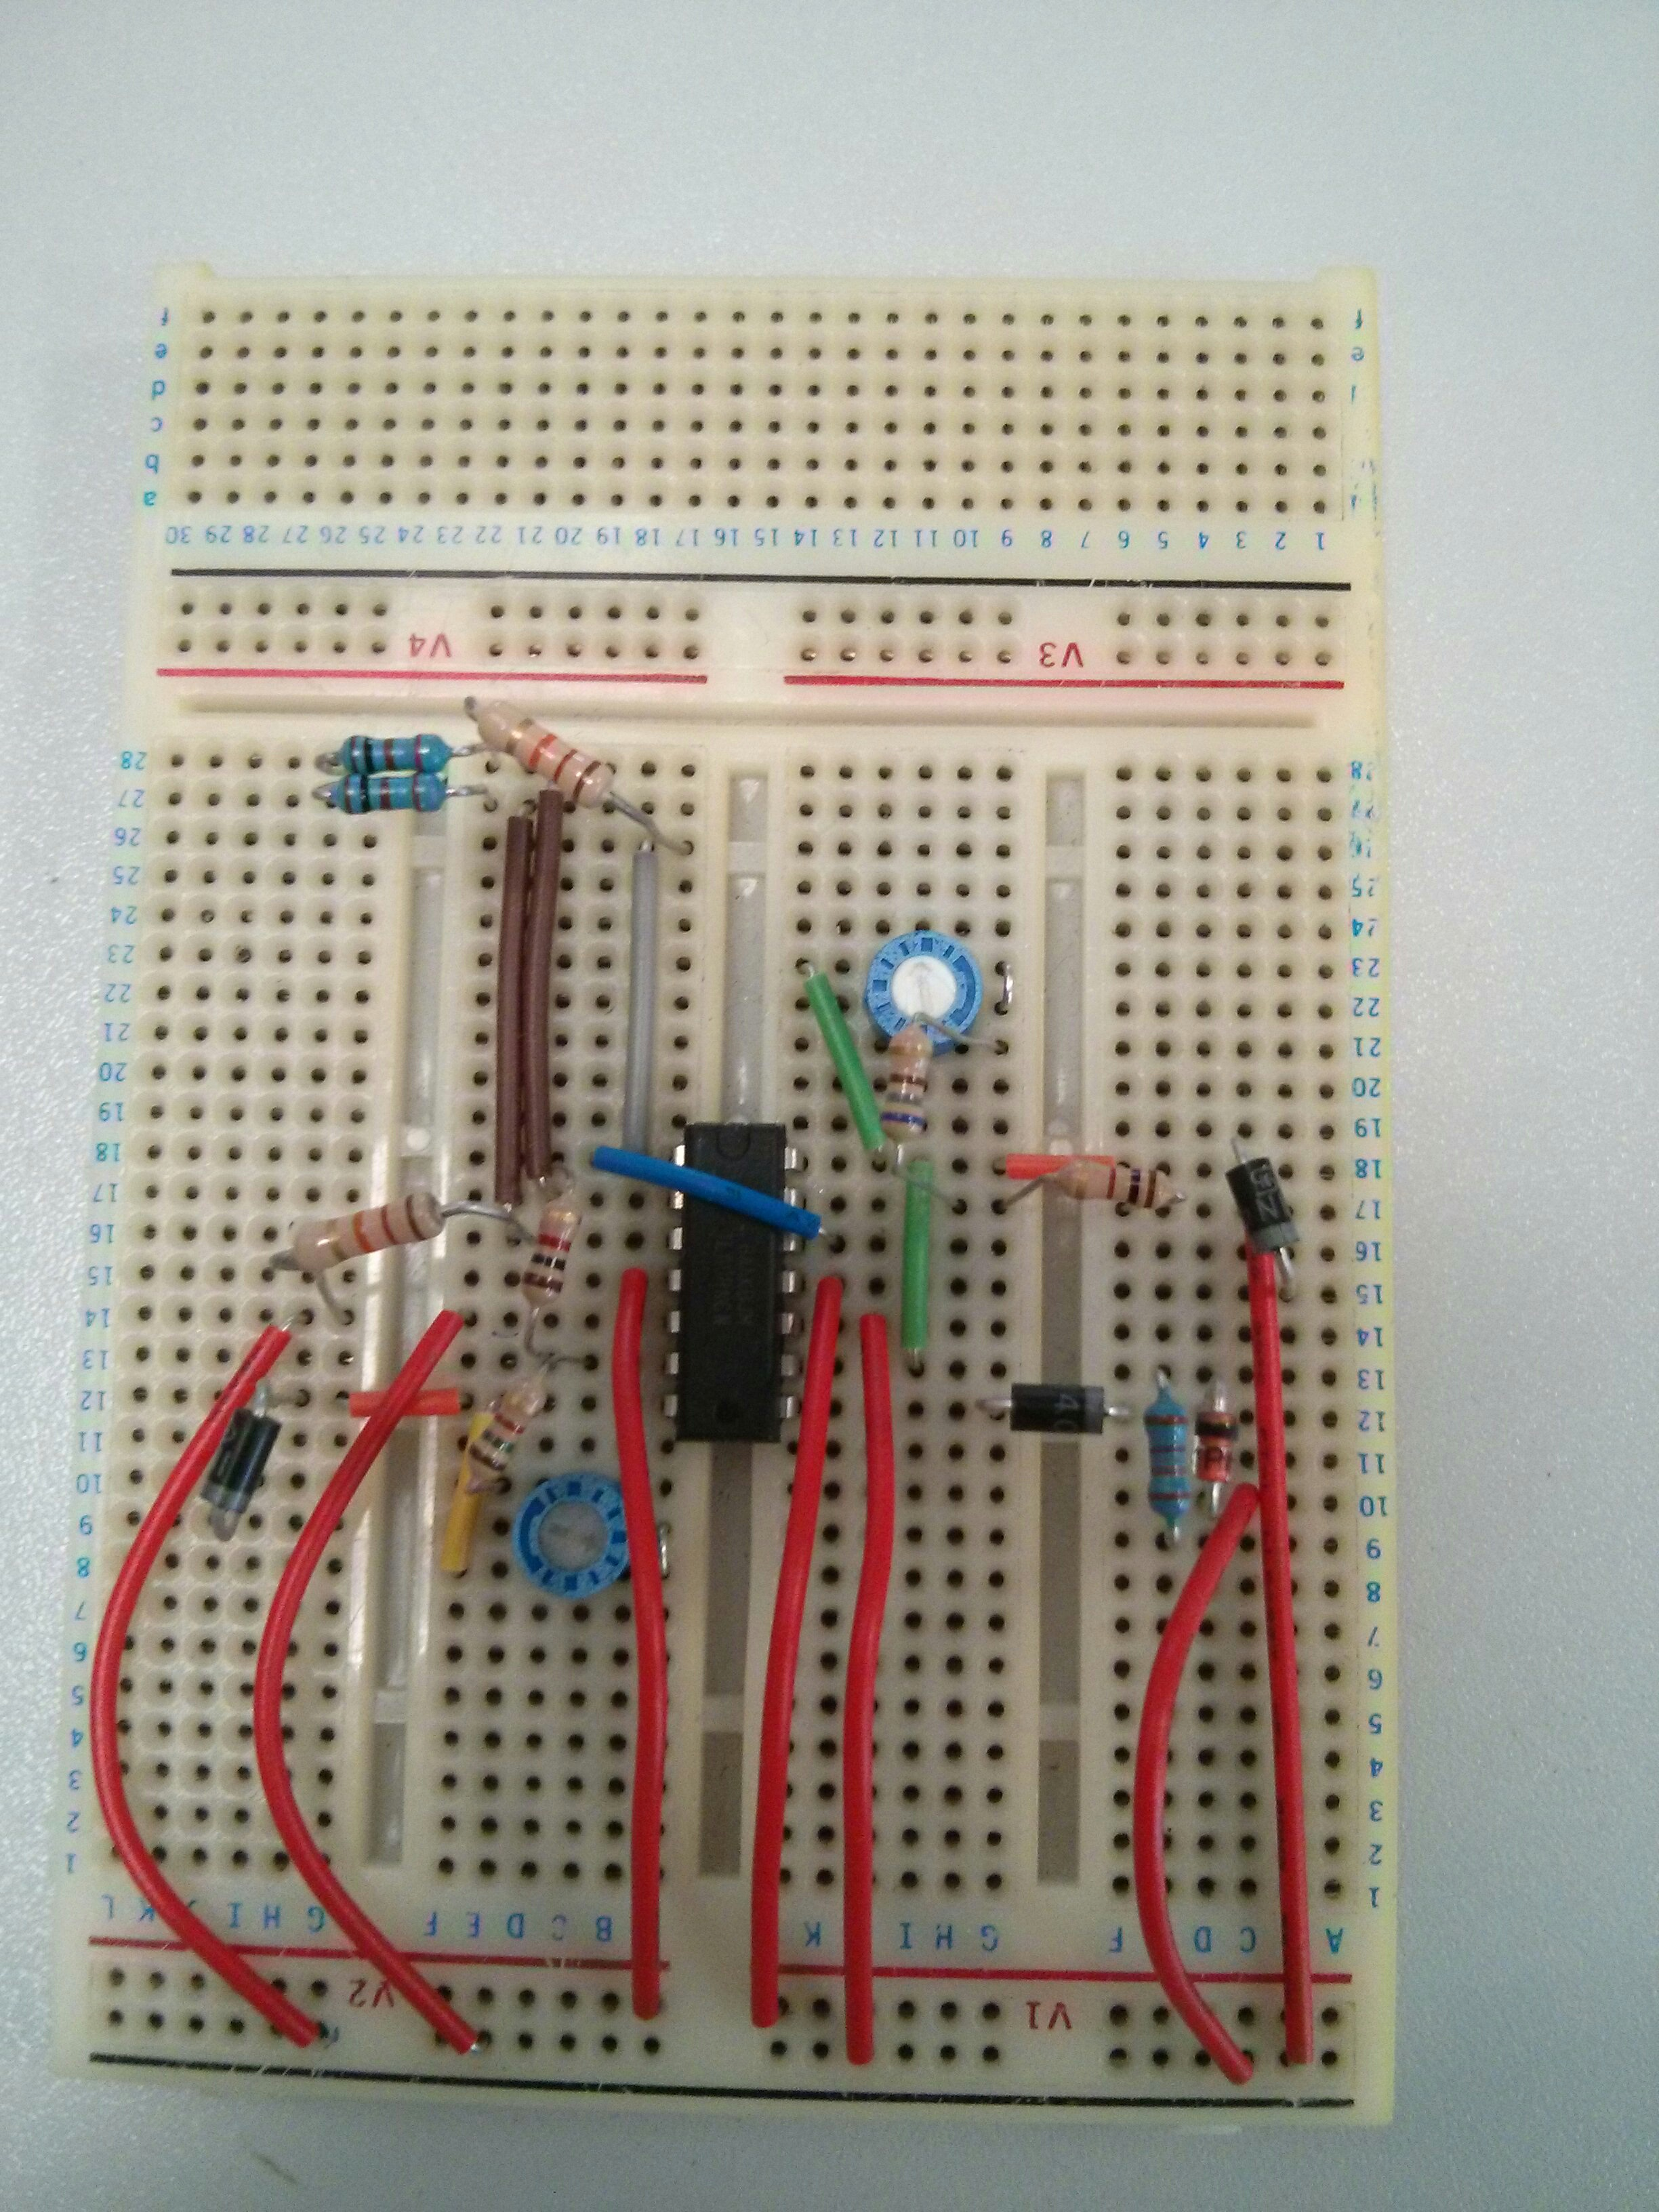
\includegraphics[width=125px]{IMG_20160629_203932.jpg}
		\end{textblock*}
		
	\end{frame}

	\section{Montage du banc d'essai}

	\begin{frame}{Banc d'essai}
		
		\begin{textblock*}{80mm}(20mm,10mm)
			\begin{itemize}
				\item Réalisation des pièces manquantes
				\item Montage de l'ensemble
				\item Câblage
 			\end{itemize}
		\end{textblock*}

		\begin{textblock*}{80mm}(25mm,35mm)
				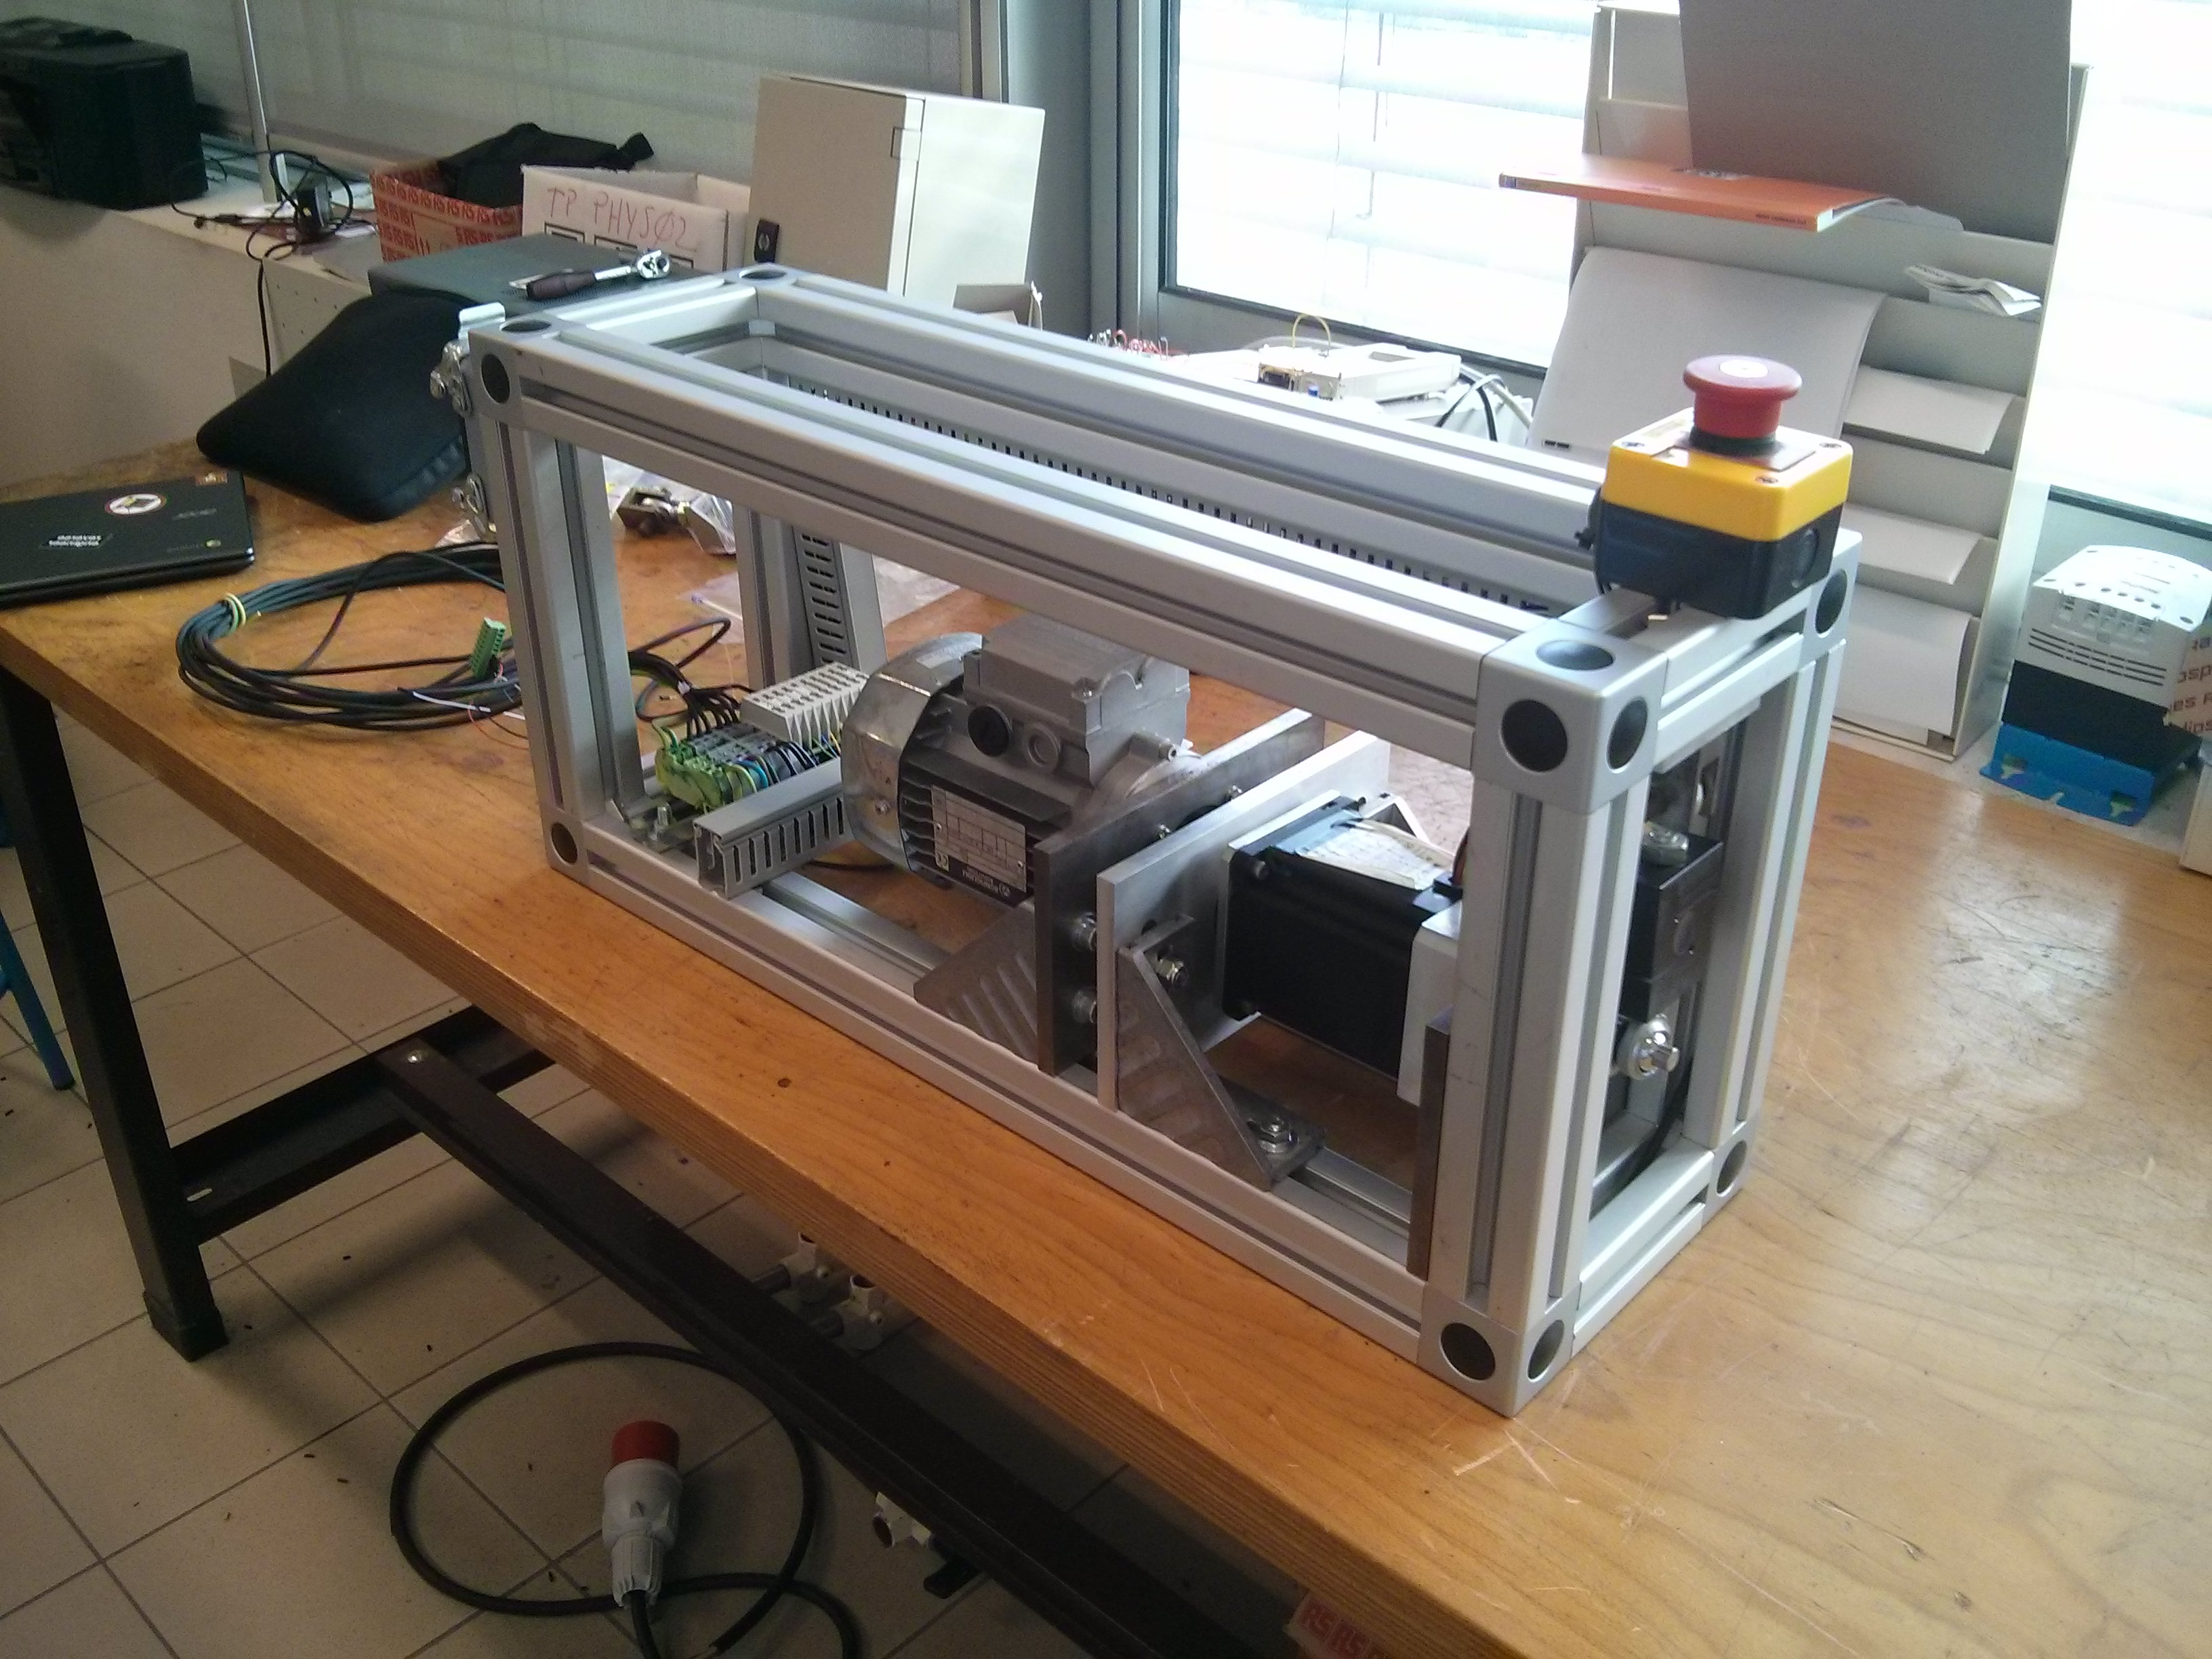
\includegraphics[width=200px]{IMG_20160628_183017.jpg}
		\end{textblock*}
		
	\end{frame}

	\begin{frame}{Armoire électrique}
		
		\begin{textblock*}{80mm}(20mm,10mm)
			\begin{itemize}
				\item Intégration de tous les éléments
				\item Câblage
 			\end{itemize}
		\end{textblock*}

		\begin{textblock*}{80mm}(25mm,25mm)
				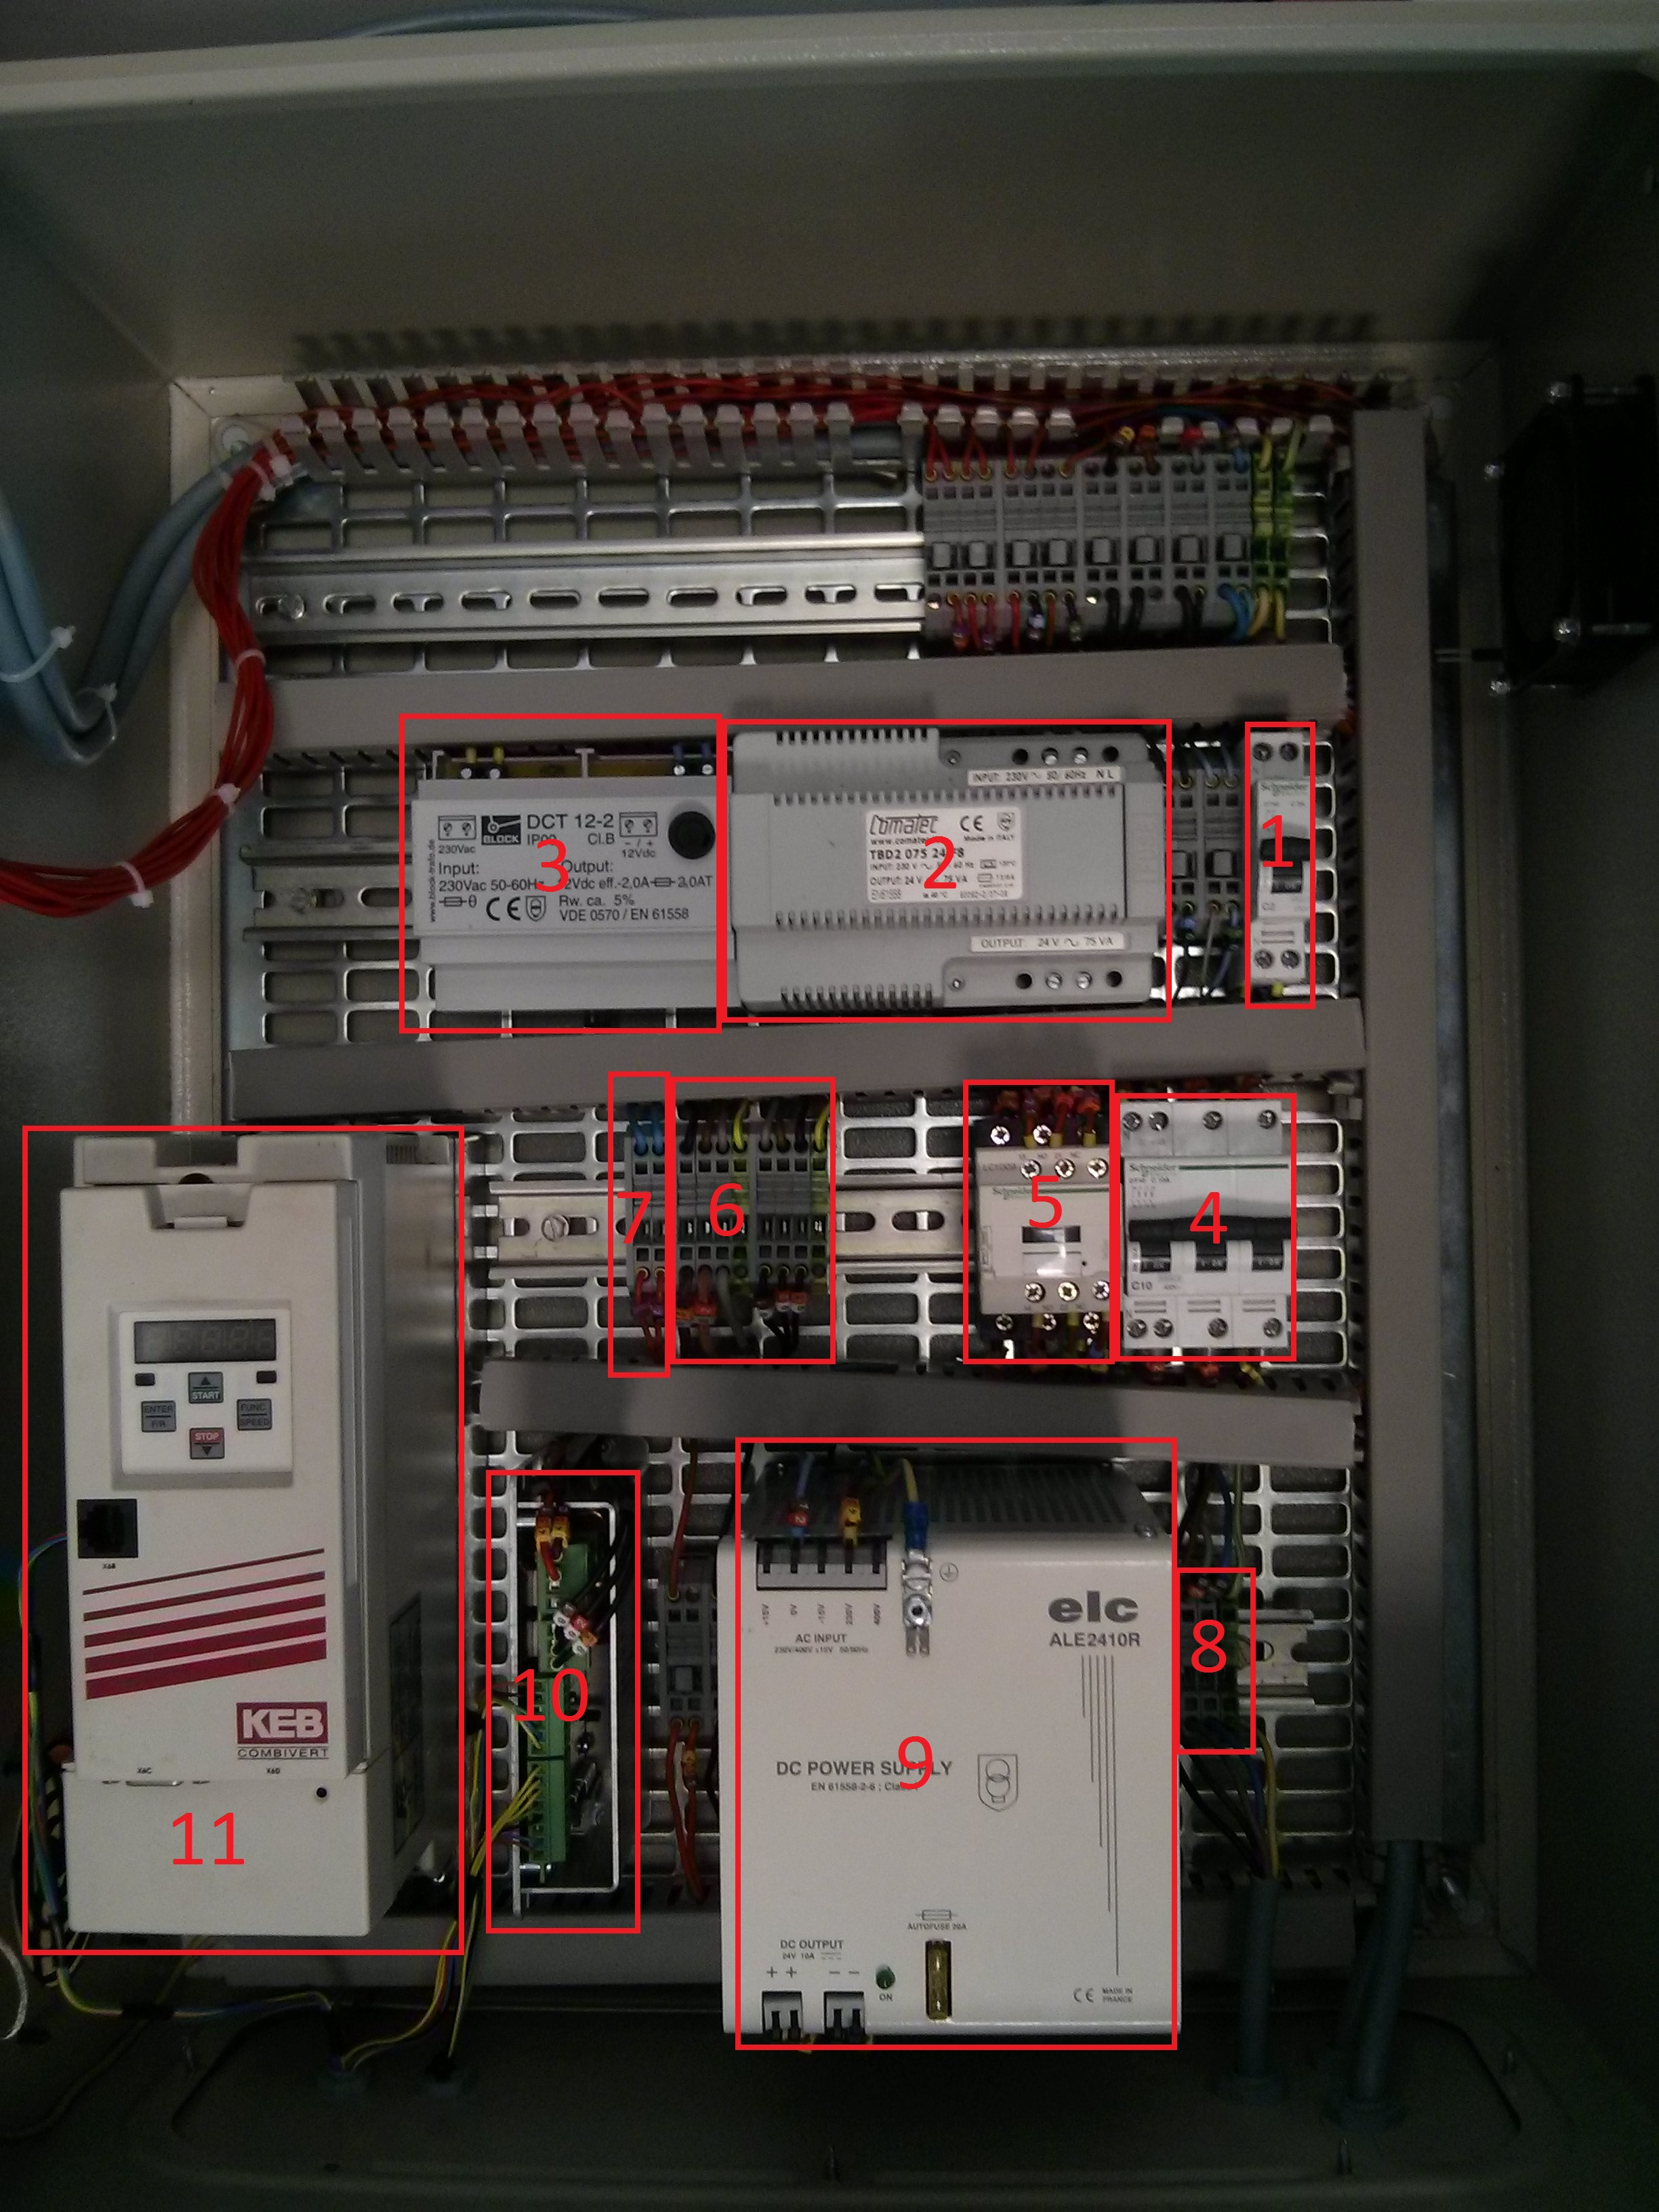
\includegraphics[width=160px]{IMG_20160629_193634.jpg}
		\end{textblock*}
		
	\end{frame}

	\section{Améliorations futures}

	\begin{frame}{Améliorations futures}
		
		\begin{textblock*}{100mm}(25mm,30mm)
			\begin{itemize}
				\item Cartérisation du banc d'essai
				\item Support pour l'armoire
				\item Achat des élements de régulation pour l'électronique
				\item Création de la carte électronique de contrôle
 			\end{itemize}
		\end{textblock*}
		
	\end{frame}

	\section{Conclusion}
	\section{Questions ?}
\end{document}